\chapter{System Design}



\section{Requirements}


\subsection{Functional Requirements}
\begin{itemize}
\item An accurate method of detecting incidents which may occur while cycling.
\item A more personalized detector, allowing better detection for riders of all abilities. 
\item As lightweight and efficient application as possible to enable compatibility with as many devices as possible, as well as reducing battery usage. 
\item Automatic SMS functionality to allow one to be located in the event of an accident.
\item Locate the rider accurately in the event of an accident as quickly as possible. 
\end{itemize}


\subsection{Non-Functional Requirements}
\begin{itemize}
\item Useful statistics computed and displayed for the user (Average Speed, Distance Travelled)
\item Google Map integration providing an accident heatmap to warn of potential dangers as well as plotting journeys.
\item A compass to help with navigation if both gps and internet connectivity are unavailable.
\end{itemize}


\newpage


\section{Interface Design}


%%%%%%%%%%%%%%%%%%%%%%%%%%%%%%%%%%%%%%%%
\begin{wrapfigure}{r}{0.5\textwidth}
\begin{center}
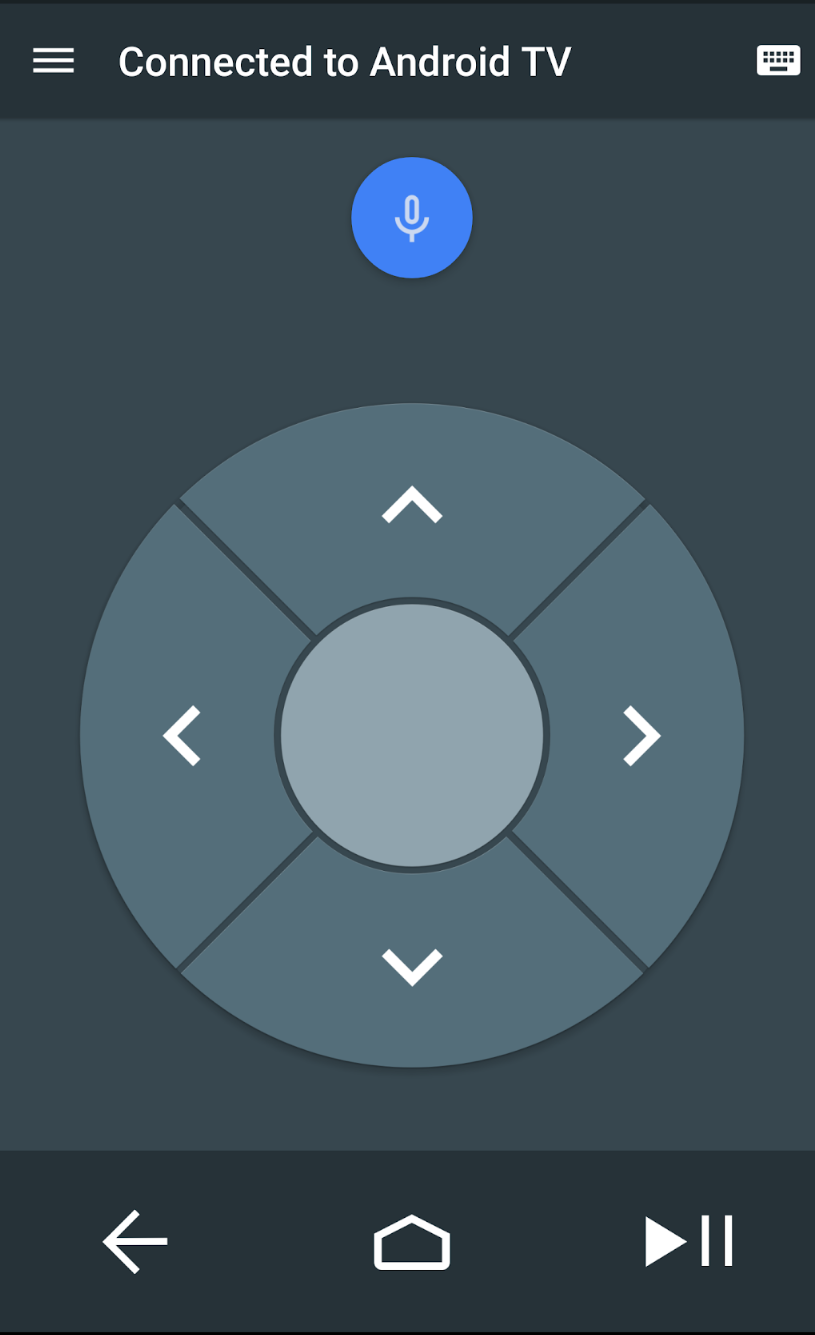
\includegraphics[scale = 0.4] {design/hs1.png}
\end{center}
\caption{Simple Home Screen Layout}
\label{hs1}
\end{wrapfigure}
%%%%%%%%%%%%%%%%%%%%%%%%%%%%%%%%%%%%%%%%

As simplicity and usability were key in the development of this application, the design of RideSafe was heavily influenced by Google's standard layout recommendations. For RideSafe functional requirements had a higher precedence than a fancy looking user interface. Inspiration was drawn from popular apps utility applications. As shown in figure \ref{hs1}  the main function of the application is the first screen the user will land on, removing extraneous steps required for the user to reach their goal - in this case change the channel. A simple uncluttered layout with only the necessary buttons required on the screen. 


%%%%%%%%%%%%%%%%%%%%%%%%%%%%%%%%%%%%%%%%
\begin{wrapfigure}{l}{0.5\textwidth}
\begin{center}
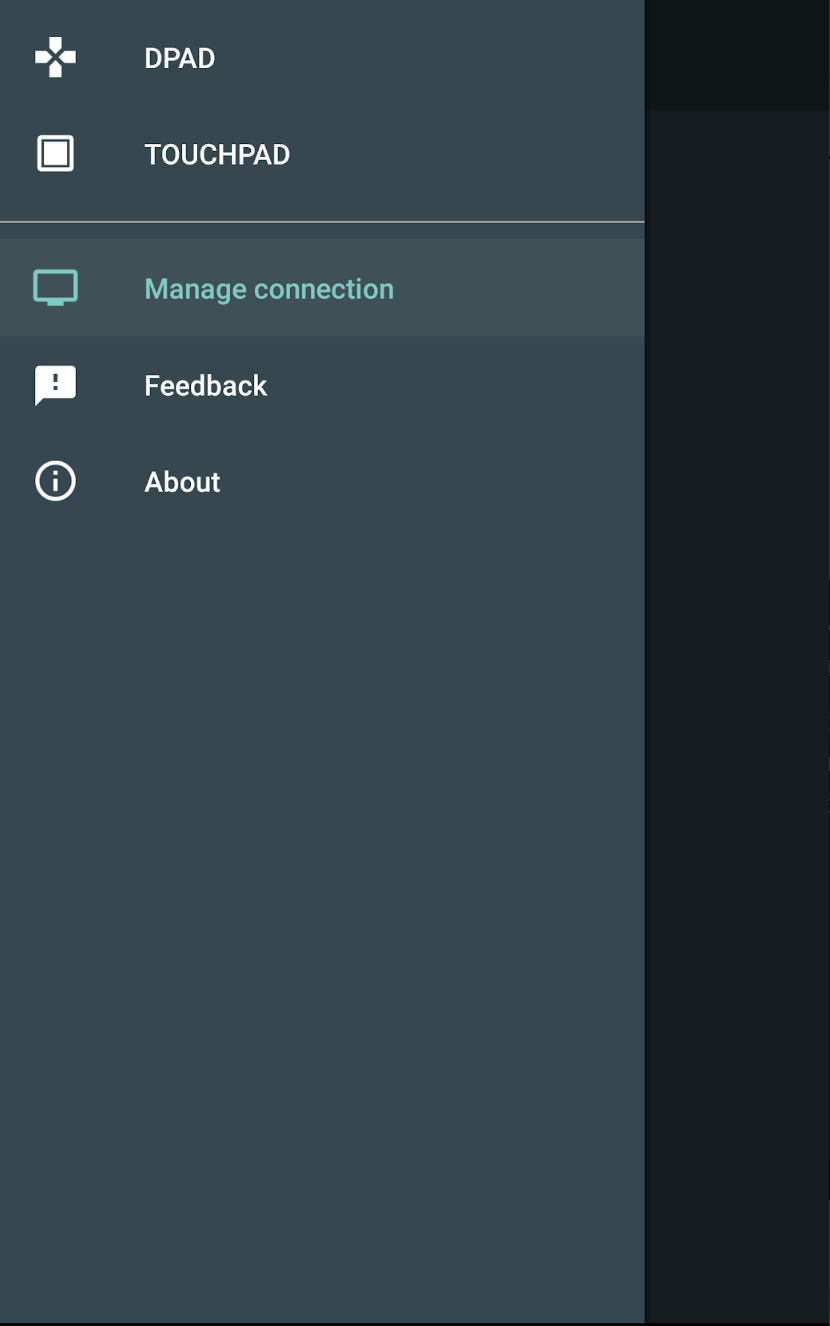
\includegraphics[scale = 0.4] {design/hme.png}
\end{center}
\caption{An Example implementation of A Navigation Drawer}
\label{hme}
\end{wrapfigure}
%%%%%%%%%%%%%%%%%%%%%%%%%%%%%%%%%%%%%%%%




For features less often used, Google's navigation drawer AKA the hamburger menu is a popular choice. As shown in figure \ref{hme} they are simple to use and allow for easy navigation to secondary functions of the application. Implementing a navigation drawer minimizes wasted space which would be taken up by adding a button for every secondary feature on the home screen, allowing the most important functionality to use up more screen real estate. As the hamburger menu is so common in every category of application on the play store, there is a high probability users will have encountered it before - resulting in a smaller learning curve to navigate through the application.


%%%%%%%%%%%%%%%%%%%%%%%%%%%%%%%%%%%%%%%%
\begin{wrapfigure}{c}{0.5\textwidth}
\begin{center}

\includegraphics[scale = .5] {design/logo.png}
\end{center}
\caption{App icon Inspiration}
\label{logo}
\end{wrapfigure}
%%%%%%%%%%%%%%%%%%%%%%%%%%%%%%%%%%%%%%%%


Colour and contrast of screen elements were a simple choice, having experience using my phone trailside in all conditions ranging from sweltering hot days to snowstorms. Simplicity is of utmost importance, glare on the screen makes any app impossible to see, especially apps featuring a dark theme.  My experience led me to favour a bright white theme with dark icons for maximum contrast. Accent colors were also an easy choice,  red was chosen as it is the color associated with “emergencies”  and “hospitals” figure \ref{logo}. Complementary shades of red were chosen using a material design palette generator \cite{color}.





\section{System Architecture Design}

This section will discuss in detail the method used to implement the crash detection logic used in RideSafe



\subsection{System Type}

Examining the vast amount of research done on fall detection in the medical domain, implementations which are threshold based could immediately be ruled out, as discussed in (section 2) threshold based solutions pose multiple issues in multiple areas, leading to the author not considering using this method.

A rule based implementation, with their proven accuracy and reliability was ultimately chosen to be the underlying architecture of ridesafe. Implementing a rule based system allows for more context to be considered measuring different data points at separate time frames, allowing the decision process to be based off a time interval rather than one moment in time. As will be discussed in the following subsection the author's choice of data points require a short period of time to determine if a crash has occurred rather than a single moment in time leading to a rule based solution to be the optimal solution.     


\subsection{Sensors \& Measurements}


Rather than just using the same data points used in existing solutions, the author launched an investigation into the suitability of different data points to determine if an accident has occurred. RideSafe Data Collection as it is now called is a logging application which was developed by the author to record multiple data points in multiple formats. While using the data collection application mountain biking over a period of a month at local trail centres. With a dataset containing tens of thousands lines of data points collected the data was visualized  and analized. For RideSafe my findings of the most relevant data points and sensors to utilize were chosen. 
\vspace{1cm}
\begin{itemize}
\item Triaxial Accelerometer
\end{itemize}


%%%%%%%%%%%%%%%%%%%%%%%%%%%%%%%%%%%%%%%%
\begin{wrapfigure}{r}{0.3\textwidth}
\begin{center}
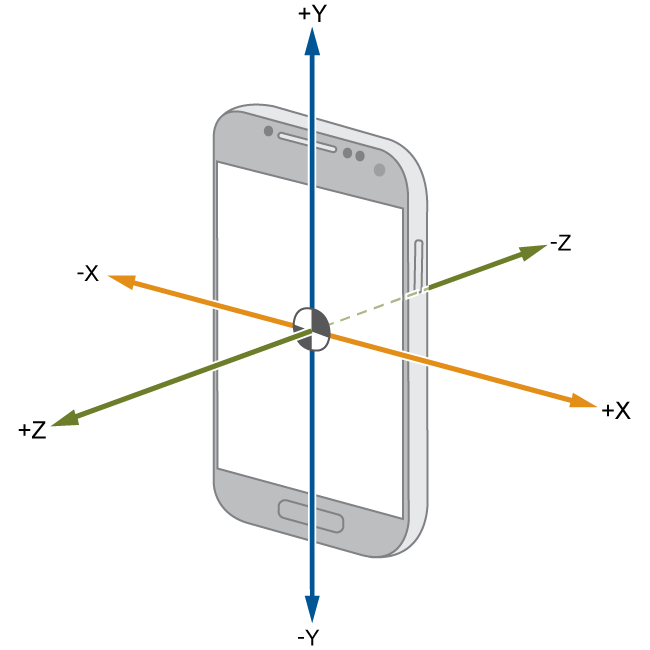
\includegraphics[scale = .2] {design/a.png}
\end{center}
\caption{Different Axis of an Accelerometer (Source Mathworks)}
\label{accel}
\end{wrapfigure}
%%%%%%%%%%%%%%%%%%%%%%%%%%%%%%%%%%%%%%%%

Like virtually every crash/fall detection solution, the triaxial accelerometer measuring linear acceleration of a body in three different axis as shown in figure \ref{accel} in \(m/s^2\). From my research the accelerometer was found to be a key sensor in determining if a crash has occurred. Using the well known Pythagorean theorem:  

\[
\mathit{} = 
\sqrt{x^2 + y^2 + z^2}
\]


  and accounting for the force of gravity on earth by subtracting  9.8 \(m/s^2\), directionless  g-force can be calculated. As the phones intended orientation is purposely unspecified directionless gforce is used to not require a certain axis to require a certain orientation.

\vspace{1cm}

\begin{itemize}
\item Triaxial Gyroscope
\end{itemize}

%%%%%%%%%%%%%%%%%%%%%%%%%%%%%%%%%%%%%%%%
\begin{wrapfigure}{l}{0.3\textwidth}
\begin{center}
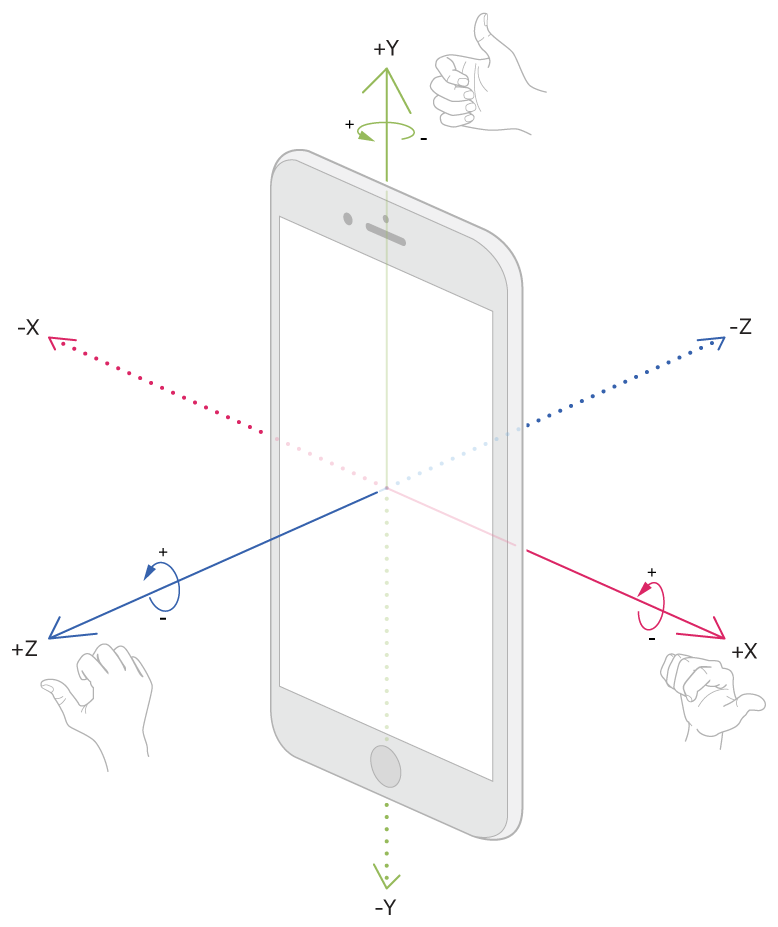
\includegraphics[scale = .1] {design/g.png}
\end{center}
\caption{Different Axis of a Gyroscope (Source Mathworks)}
\label{gyro}
\end{wrapfigure}
%%%%%%%%%%%%%%%%%%%%%%%%%%%%%%%%%%%%%%%%


The use of android's built in gyroscope allows for measuring rotational acceleration in three different axes as shown in figure \ref{gyro}. To measure rotational force in a certain direction the phone's orientation must be known, in this case where the orientation is unspecified total change in rotational acceleration was chosen, measuring the change in total rotation rather than on a per axis basis. The difference of the combined change in rotational acceleration is what the author found to be the most suitable reading. 
\vspace{1cm}

\begin{itemize}
\item Speed - GPS
\end{itemize}

From the authors investigation the change of speed was of great importance as a datapoint to consider. Many existing solutions for cycling re-use the logic found in fall detection for the elderly, a system designed to work indoor where speed isn't much of a factor. The author found that change of speed was directly related to a crash occurring as well as other activities. 

\vspace{2cm}
%%%%%%%%%%%%%%%%%%%%%%%%%%%%%%%%%%%%%%%%
\begin{figure}[h]
	\centering
	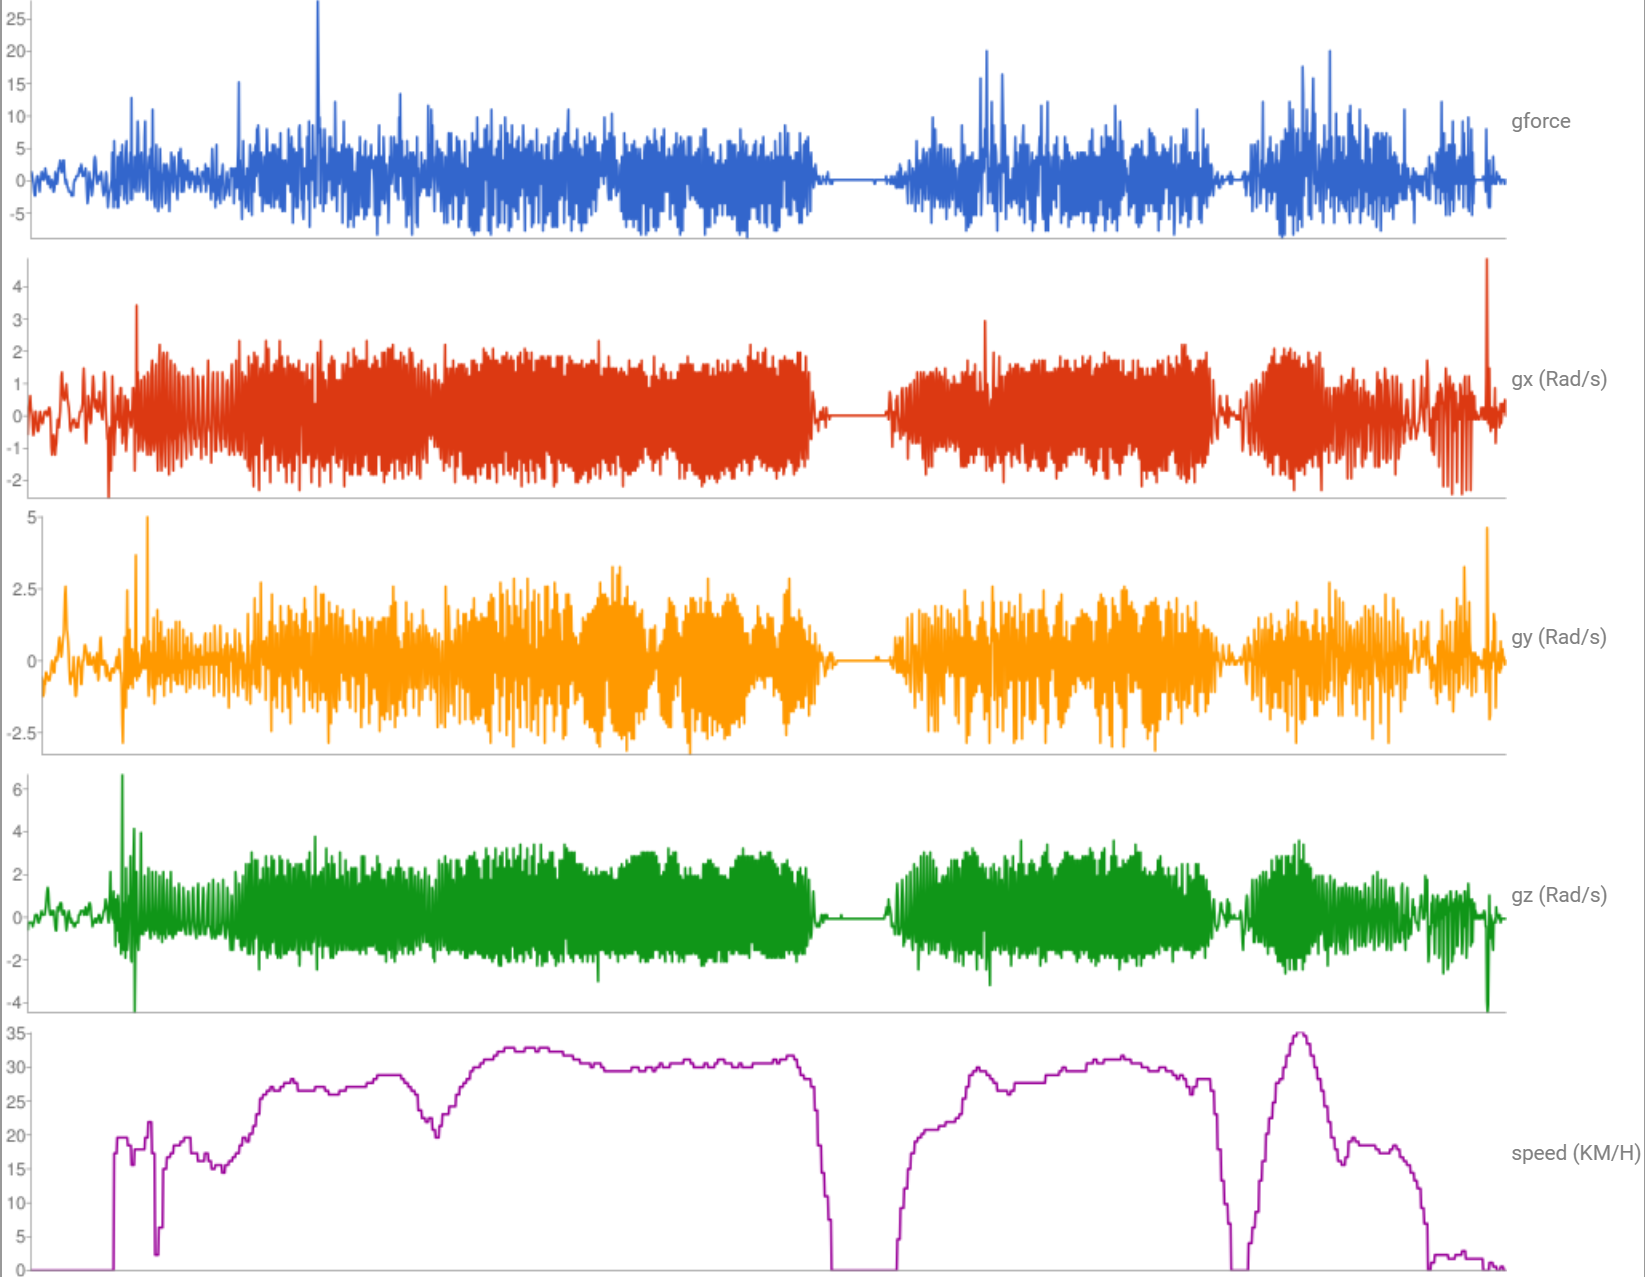
\includegraphics[scale = .7] {design/sampledata.png}
	\caption{G-Force, Angular Velocity and Speed  over time}
	\label{sampledata}
\end{figure}
%%%%%%%%%%%%%%%%%%%%%%%%%%%%%%%%%%%%%%%%
\vspace{1cm}

Figure \ref{sampledata} shows data collected from RideSafe data collection during a cycle in the Dublin mountains. The data represents a normal mountain bike spin on metro 1, spikes of g-force can be observed, as a result of landing jumps or simply a rough section of the trail. The large decreases in speed throughout the data are a result of extremely tight corners and or quick rests in between.

\newpage

\section{Machine Learning}



With this design we have multiple continuous variables to consider to determine if a crash has occurred.  Given the multiple current data values a probability needs to be computed. Using supervised machine learning outcome predictions can be made for given values once the model is trained with sufficient examples of both positive and negative examples. Researching commonly used machine learning techniques used in fall detection \cite{commonSolutions}, the author considered two possible methods. 
\begin{itemize}
\item Support vector machines (SVM)
\item Logistic Regression(LR)
\end{itemize}
Both SVM and (LR) are algorithms commonly used for classification, both performing comparably in practice. The main goal of both (LR) \& (SVM) are to calculate the best fitting line of divide in a given dataset, allowing for predictions to be made using similar data. SVM’s maximize the “line” of fit using support vectors maximizing the margin producing a class divide, outputting  a binary value 1 or 0 depending on class membership. LR using a sigmoid function outputs probabilities of a value belonging to class 1 between 0 and 1. LR allows for a manual class divide line to be set enabling a desired probability to set for the class divide. Logistic Regression's accuracy has been previously evaluated with both balanced and imbalanced data leading to accuracy exceeding 90\% in both cases \cite{suit}. Having previously studied Logistic regression paired with promising accuracy with test values, the author decided on basing the implementation on Logistic Regression due to the flexibility of the algorithm as well its simplicity to implement in java.


























